\documentclass[msc,    % ou [msc] para dissertações 
  % hidetitle,         % de mestrado. Para propostas ou
  hidecover,           % projetos, usar [phd,project],
  hidefc,              % [msc,proposal], etc.
  hideapproval,
  hideack,
  a4paper
  ]{ppgccufmg} 

\usepackage[brazil]{babel}        % se o documento for em português, OU
%\usepackage[english]{babel}      % se o documento for em inglês
\usepackage[utf8x]{inputenc}
\PrerenderUnicode{ã}
\usepackage[T1]{fontenc}
\usepackage{type1ec}
\usepackage{graphicx}
\usepackage{multirow}
\usepackage{listings} % escrever trechos de códigos
\usepackage{xcolor}
\lstset { %
  language=C++,
  backgroundcolor=\color{black!5}, % set backgroundcolor
  basicstyle=\footnotesize,% basic font setting
  showstringspaces=false,
}
\usepackage{subcaption} % subfigures
\usepackage{amssymb,amsmath} % equações

\usepackage[portuguese,
  bookmarks=true,
  bookmarksnumbered=true,
  linktocpage,
  colorlinks,
  citecolor=black,
  urlcolor=black,
  linkcolor=black,
  filecolor=black
  ]{hyperref}
\usepackage[square]{natbib}
\usepackage{ltxtable, tabularx, longtable}
\usepackage{booktabs}% http://ctan.org/pkg/booktabs
\newcommand{\tabitem}{\textbullet~}

\begin{document}

% O comando a seguir, \ppgccufmg, provê todas as informações relevantes para a
% classe ppgccufmg. Por favor, consulte a documentação para a descrição de
% cada chave.

% Um exemplo para documentos em português é apresentado a seguir:
\ppgccufmg{
  title={Método Automático de Contagem Volumétrica de Veículos baseado em Visão Computacional},
  authorrev={Ferreira Bailão, Arthur},
  % cutter={D1234p},
  % cdu={519.6*82.10},
  university={Universidade Federal de Minas Gerais},
  course={Engenharia de Controle e Automação},
  address={Belo Horizonte},
  date={2014-11},
  keywords={Visão Computacional, Engenharia de Transporte, Contagem Volumétrica},
  advisor={Prof. Hermes Aguiar Magalhães},
  supervisor={Profª. Leise Kelli de Oliveira},
%  approval={img/approvalsheet.eps},
%  approval=[-2.5cm][1]{aprovalsheet},
  abstract={Resumo}{abstract_ptbr},
  abstract=[english]{Abstract}{abstract_en},
  % abstract={Resumo Estendido}{resumoest},
  % dedication={dedication},
  % ack=[Acknowledgments]{thanks},
% ack=[Acknowledgments]{ack},
  epigraphtext={A ciência pode ser descrita como a arte da sistemática simplificação.}{Karl Popper}
}

\chapter{Introdução} % (fold)
\label{cha:introdu_o}
% !TEX root = pfc.tex

O tráfego de veículos representa um fenômeno de grande importância socioeconômica, principalmente nos grandes centros urbanos cujos deslocamentos, no menor tempo possível, são uma necessidade cotidiana. Projetar sistemas viários que absorvam toda a frota veicular desses grandes centros e minimizam os congestionamentos exige ferramentas cujo desenvolvimento ainda representa objeto de estudo para diversos grupos de pesquisadores.

Vários fatores interferem na qualidade do tráfego, sendo o principal o crescente número de veículos nos centros urbanos. Segundo \cite{fenabrave:2013:online} - Federação Nacional da Distribuição de Veículos Automotores, as vendas de veículos cresceram cerca de 381\% entre janeiro de 2003 e janeiro de 2011. A facilitação ao crédito pessoal, os longos financiamentos oferecidos pelas concessionárias e a redução do IPI (Imposto sobre Produtos Industrializados) incentivaram o consumo de carros no Brasil, explicando essa tendência ascendente no número de automóveis.

% \begin{figure}[tb]
%   \begin{center}
%     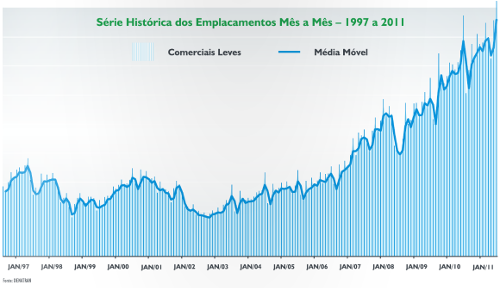
\includegraphics[scale=0.8]{imgs/emplacamentos.png}
%   \end{center}
%   \caption{Crescimento mensal no número de emplacamentos de veículos comerciais leves no período 1997 a 2011 \citep{fenabrave:2013:online}.} 
%   \label{fig:fenabreve}
% \end{figure}

A falta de planejamento urbano e o crescente aumento de veículos, a péssima qualidade do transporte público no Brasil e o excessivo número de acidentes de trânsito são umas das principais causas de congestionamentos. Nos últimos anos, milhões de pessoas perderam tempo e dinheiro devido a problemas relacionados ao trânsito \citep{pamela:2012:masther}. Diante desse fato, a administração pública deve priorizar o assunto mobilidade, como tem sido feito nas principais regiões metropolitanas brasileiras. Através de pesquisas pode-se levantar dados que contribuem para análise e simulação do tráfego. Informações como fluxo de veículos, volume de tráfego e matriz O/D (origem/destino) são de grande relevância no estudo dessa área, formando uma base teórica sólida para ser utilizada na resolução de problemas dessa natureza.

Na área de simulação do tráfego existem várias empresas atuantes: \cite{vissim:2013:online} é atualmente a líder mundial de mercado em simulação de fluxo de tráfego multi-modal de microregiões. Outras companhias, \cite{arcady:2013:online} e \cite{citilabs:2013:online}, também fornecem produtos com capacidades de predição, simulação de congestionamentos, atrasos, acidentes, além de gerar relatórios detalhados e animações 2D e 3D. SUMO - \textit{Simulation of Urban MObility} é uma alternativa \textit{open source}\footnote{O termo código aberto, ou \textit{open source} em inglês, foi criado pela OSI e refere-se a \textit{software} livre. Mais informações em \url{http://opensource.org}} e gratuita para simulação do tráfego, diferente dos produtos proprietários e de alto custo citados anteriormente \citep{SUMO2011}.

Segundo \cite{dnit:2011:online}, o PNCT - Plano Nacional de Contagem de Trânsito vem armazenando nos últimos anos importantes dados de volume de tráfego e já possui uma significativa série histórica desses dados. A informação coletada é de grande importância pois seus resultados são subsídios básicos para estudos econômicos, projetos rodoviários e planejamento de tráfego, além do papel essencial no estabelecimento de critérios para o cumprimento das seguintes finalidades:

\begin{itemize}
  \item Planejar o sistema rodoviário;
  \item Programar necessidades e prioridades de melhorias no sistema rodoviário;
  \item Estabelecer as tendências de tráfego no futuro;
  \item Avaliar o fluxo existente de tráfego em relação ao sistema rodoviário atual;
  \item Justificar e planejar o policiamento;
  \item Estudos de localização de postos de pesagem, socorro médico emergencial, etc.;
  \item Projetar pavimento, obras de arte, seção transversal e outros elementos de rodovia \citep{dnit:2011:online}. 
\end{itemize}

Existem métodos manuais e automáticos para realização das contagens volumétrica e classificatória, que normalmente são de alto custo financeiro. De acordo com a forma de instalação dos equipamentos de contagem, tais métodos podem ser invasivos ou não-invasivos. Os métodos invasivos necessitam de instalações junto ou sob a camada asfáltica. Já os métodos não-invasivos normalmente utilizam câmeras, sensores ou instalações sobre o solo \citep{goldner:2009:misc}.

Este trabalho tem como propósito desenvolver um método computacional de simples implementação, configuração, instalação e operação, capaz de realizar a contagem volumétrica de veículos de forma não-invasiva e que possa ser utilizado como uma alternativa de baixo custo financeiro, se comparado aos sitemas de contagem volumétrica convencionais.

\section{Objetivos} % (fold)
\label{sec:objetivos}

O objetivo principal do trabalho é desenvolver um sistema de visão computacional que auxilie na análise das condições do tráfego urbano. São os objetivos específicos deste estudo:
\begin{itemize}
  \item Entender a utilização de um sistema de visão para problemas de transporte;
  \item Realizar a contagem volumétrica dos veículos através de um método não-invasivo de simples implementação;
  \item Analisar as condições do tráfego urbano através de imagens coletadas por uma câmera digital;
  \item Através da análise dos resultados, determinar a qualidade do método e identificar pontos de acerto e erro que podem ser trabalhados.
\end{itemize}

% section objetivos (end)

% \section{Apresentação da Empresa} % (fold)
% \label{sec:apresenta_o_da_empresa}

% TODO: não é mais empresa

% A NunesCV é uma startup que foi criada no início de 2013 e desenvolve soluções e produtos de tecnologia para o setor de serviços. A empresa desenvolve sistemas baseados em visão computacional, como um produto para leitura automática de cartões de ponto utilizando tecnologia própria de Reconhecimento Ótico de Caracteres (OCR).

% Outro tipo de aplicação desenvolvida pela empresa é um sistema de gerenciamento remoto de uma rede de mídia indoor, que são televisões instaladas em pontos comerciais estratégicos anunciando informações úteis para os usuários. Cada ponto pode ter o conteúdo atualizado em tempo real via Internet, além de informar se a televisão está ligada e se o conteúdo está correto. A empresa desenvolve o software para um sistema embutido que controla o aparelho, o sistema web de gerenciamento e atualização de conteúdo e especifica o hardware necessário para o funcionamento do sistema.

% section apresenta_o_da_empresa (end)

\section{Organização do Texto} % (fold)
\label{sec:organiza_o_do_texto}

A monografia está dividida em seis capítulos:

\begin{itemize}
  \item Capítulo \ref{cha:introdu_o} é introdutório e são apresentados alguns pontos que motivam e justificam o desenvolvimento do projeto, além de uma listagem dos objetivos específicos que definem o escopo do mesmo.
  \item Capítulo \ref{cha:contagem_de_ve_culos_e_monitoramento_do_tr_fego} apresenta as tecnologias de contagem volumétrica e classificatória existentes. É também apresentado uma pesquisa bibliográfica sobre sistemas de visão computacional inseridos no contexto da Engenharia de Transporte.
  \item Capítulo \ref{cha:vis_o_computacional} introduz a teoria de visão computacional, contextualizando o leitor. Trata-se de uma apresentação da tecnologia com foco em conceitos e técnicas de processamento de imagens.
  \item Capítulo \ref{cha:metodologia} apresenta a metodologia para contagem volumétrica automática de veículos. As técnicas utilizadas, a sequência de operações, as imagens de processamento, as condições de captura, a estrutura do software e os métodos para análise de resultados são mostrados e explicados. 
  \item Capítulo \ref{cha:testes_e_resultados} apresenta os resultados e a validação das contagens; uma análise crítica do método proposto mostrando como as características da cena influenciam no resultado. 
  \item Capítulo \ref{cha:conclus_o} são feitas as conclusões e as considerações finais do trabalho, bem como recomendações para trabalhos futuros.
\end{itemize}


% section organiza_o_do_texto (end)
% chapter introdu_o (end)

\chapter{Contagem de Veículos e Monitoramento do Tráfego} % (fold)
\label{cha:contagem_de_ve_culos_e_monitoramento_do_tr_fego}
% !TEX root = pfc.tex

De acordo com \cite{dnit:2011:online}, Departamento Nacional de Infra-Estrutura de Transportes, a contagem volumétrica consiste em quantificar o volume de veículos que trafegam por um determinado trecho da rodovia, durante um intervalo de tempo definido. A contagem de veículos é importante para o cumprimento de diversas finalidades, dentre elas: planejamento do sistema rodoviário, estabelecimento de tendências de tráfego futuro, determinação do volume de viagens de forma a proporcionar justificativa econômica aos investimentos programados, avaliação do fluxo existente de tráfego em relação ao sistema rodoviário atual, planejamento e justificativa do policiamento, realização de análise estatística de acidentes, estudos de localização de postos de pesagem, socorro médico emergencial, entre outros.

O volume de veículos, obtido através da contagem, pode ser classificado como \citep{goldner:2009:misc}:

\begin{itemize}
  \item \textbf{Volume de tráfego}: quantidade de veículos em tráfego na seção de uma via, em um período de tempo definido;
  \item \textbf{AADT} ou \textbf{VMDA}: volume médio diário de veículos durante o ano, ou seja, a somatória anual, dividido por 365;
  \item \textbf{ADT} ou \textbf{VMD}: volume diário do tráfego ou volume médio diário. Também é usado para intervalos de tempo diferentes, representando o volume total durante dado período, dividido pela quantidade de dias do período. Assim tem-se:
  \begin{itemize}
    \item \textbf{VMDm}: volume médio diário mensal. Número total de veículos em um mês, dividido pelo número de dias do mês;
    \item \textbf{VMDs}: volume médio diário semanal. Número total de veículos em uma semana, dividido por 7. É sempre acompanhado pelo nome do mês a que se refere;
    \item \textbf{VMDd}: Volume médio diário em um dia de semana. Deve ser sempre acompanhado pela indicação do dia de semana e do mês correspondente;
  \end{itemize}
  \item \textbf{Composição do tráfego}: porcentagem dos diferentes tipos de veículos que compõem o tráfego, por exemplo, automóveis, caminhões, ônibus e motos;
  \item \textbf{Volume abreviado}: volume do fluxo de um período menor do que 1 hora;
  \item \textbf{Variações do volume de tráfego}: mudanças no volume em um determinado período, divididas em: variações sazonais ou mensais ao longo do ano; variações diárias ao longo da semana; variações horárias ao longo do dia; e variações dentro da hora.
\end{itemize}

\cite{goldner:2009:misc} define dois métodos de contagem: \textbf{manual} e \textbf{mecânica}. A contagem manual utiliza recursos humanos, ou seja, pesquisadores observam o fluxo de veículos e manualmente fazem suas anotações. Esse procedimento é vantajoso pela precisão e variedade nas informações de tráfego obtidas, como tipo e tamanho dos veículos, além de proporcionar flexibilidade, simplicidade e rapidez de execução. No entanto, é um método com limitações de cobertura e de alto custo. A contagem mecânica utiliza detectores de tráfego de instalações permanente ou móvel. Possui algumas vantagens, dentre elas: baixo custo operacional, grande amplitude de tempo de cobertura e boa precisão. Por outro lado não fornecesse muitas informações e demanda investimento inicial alto.

A classificação feita por \cite{goldner:2009:misc} peca ao usar o termo contagem mecânica para caracterizar métodos não manuais. Grande parte dos equipamentos de contagem volumétrica são dispositivos eletrônicos, por exemplo sensores micro-ondas, ultra-sônicos e piezoelétricos, descaracterizando o uso dessa nomenclatura. Até mesmo o tubo pneumático, que pode ser considerado um dispositivo mecânico, utiliza sinais elétricos para transmissão dos dados. Por esse motivo, será adotado o termo \textbf{contagem automática} para descrever os métodos de contagem que não dependem diretamente da participação humana durante o processo de obtenção dos dados.

Por sua vez, os métodos automáticos de contagem podem ser classificados como \textbf{invasivos} e \textbf{não-invasivos}. Os métodos invasivos necessitam de instalações junto ou sob a camada asfáltica. Já os métodos não-invasivos não modificam a estrutura da via, com instalações acima ou às margens da faixa de tráfego \citep{goldner:2009:misc}.

Nas seções seguintes são apresentados alguns equipamentos automáticos de contagem volumétrica, descritos em \cite{goldner:2009:misc}, \cite{almeida:2010:masther} e \cite{dnit:2011:online}, bem como algumas aplicações de visão computacional inseridas na área de Engenharia de Transporte.

\section{Tecnologias detectoras de veículos} % (fold)
\label{sec:tecnologias_detectoras_de_ve_culos}

Atualmente existem diversas tecnologias de sensores capazes de efetuar a detecção de veículos \citep{minnesota1997field}. A Tabela \ref{tab:tecnologias_vantagens_desvantagens} lista grande parte delas, apresentando vantagens e desvantagens para cada uma \citep{aguiar2008thesis}. Nas subseções a seguir alguns sensores que utilizam essas tecnologias são detalhados.

\LTXtable{\textwidth}{advantages_disadvantages}

\subsection{Detector de laço indutivo} % (fold)
\label{sub:detectores_de_la_os_indutivos}

São os sensores mais utilizados para a coleta de dados de tráfego. É composto basicamente por um circuito elétrico oscilador, uma unidade eletrônica de processamento, cabos de transmissão e o laço indutivo propriamente dito, que é formado por uma ou mais voltas de um cabo isolado instalado sob o pavimento da via (Figura \ref{fig:laco_indutivo}), caracterizando-o como equipamento invasivo.

\begin{figure}[ht]
  \begin{center}
    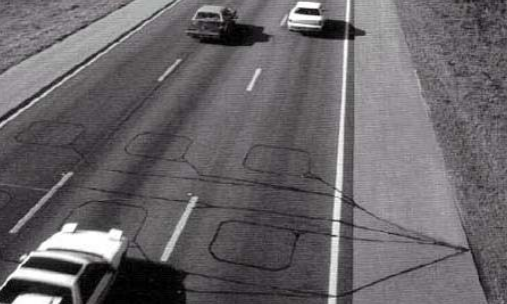
\includegraphics[scale=0.6]{imgs/laco_indutivo.png}
  \end{center}
  \caption{Seis laços indutivos instalado em uma rodovia, dois por faixa \citep{goldner:2009:misc}.}
  \label{fig:laco_indutivo}
\end{figure}

O laço funciona como indutor de um circuito oscilador de frequência fixa, normalmente entre 10 KHz e 200 KHz. Quando objetos de metal transitam nas proximidades do equipamento instalado no solo, acontece uma interação entre os campos magnéticos induzidos no laço e no objeto metálico, que normalmente é um veículo, provocando variações na indutância do laço e, portanto, variações na frequência de oscilação do circuito ressonante. A presença de um veículo na região do laço provoca um aumento na frequência de oscilação do circuito, comportamento que é interpretado pela unidade de processamento capaz de realizar a contagem.

Cada veículo que passa pelo laço indutivo possui um perfil magnético característico que depende de vários fatores, dentre eles, seu tamanho, formato, condutividade e orientação em relação ao laço. Isso possibilita, além da contagem, realizar uma classificação veicular através de métodos de clusterização por redes neurais, como descrito em \citep{almeida:2010:masther}.

A vantagem de se usar laços indutivos para monitoramento é o bom funcionamento na captura de dados básicos do tráfego, como volume e velocidade, além de apresentar baixo custo se comparado à equipamentos não-invasivos. Por outro lado, o processo de instalação do equipamento junto ao solo gera a paralisação no tráfego local e muitas vezes causa transtornos no trânsito.

% section detectores_de_la_os_indutivos (end)

\subsection{Tubo pneumático} % (fold)
\label{sub:tubo_pneum_tico}

Os sensores de contagem volumétrica por tubo pneumático funcionam a partir da pressão exercida pelos pneus de um veículo assim que passam sobre o tubo de borracha. A massa de ar é então deslocada ao longo do tubo até o ponto de conversão, onde um interruptor converte o sinal pneumático em sinal elétrico, para que esse possa ser transmitido a um \textit{software} de análise ou a um contador.

O tubo é instalado sobre a via, perpendicular à direção do fluxo do tráfego, caracterizando-se como um equipamento invasivo. É normalmente utilizado para contagem de tráfego em períodos curtos, classificação dos veículos por número de eixos e espaçamento, medição de velocidade e pesquisas acadêmicas.

Apesar de ser a primeira tecnologia de detecção de tráfego, inventada em 1920, é ainda muito utilizada devido ao baixo custo e a simples instalação e operação. No entanto, o equipamento é impreciso na contagem de caminhões ou ônibus muito largos, além de apresentar baixa durabilidade e sensibilidade à temperatura.

% section tubo_pneum_tico (end)

\subsection{Sensor magnético} % (fold)
\label{sub:sensores_magn_ticos}

O princípio de funcionamentos dos sensores magnéticos é baseado em variações das linhas de fluxo do campo magnético terrestre. Tal efeito é conhecido como anomalia magnética, causada pela aproximação de objetos metálicos (veículos) da área de cobertura do sensor. Por indução eletromagnética, variações de tensão são geradas e posteriormente amplificadas, digitalizadas e finalmente transmitidas ao controlador eletrônico que realiza a contagem.

São utilizados para medir volume, direção, presença e velocidade dos veículos. Podem ser divididos em dois tipos: os magnetômetros de indução, que se baseiam em mudanças nas linhas de fluxo do campo magnético devido ao movimento, não detectam veículos parados na via; e os magnetômetros de eixo duplo, que detectam mudanças nos componentes horizontais e verticais do campo magnético terrestre de acordo com a densidade do metal do veículo, e são capazes de identificar objetos em movimento ou parados.

 A utilização destes sensores é vantajosa devido a pouca sensibilidade à temperatura ambiente e ao tráfego intenso. Suas desvantagens são a pequena zona de detecção, a dificuldade em considerar veículos parados e a sua característica de instalação invasiva, fazendo-se necessárias paralizações do tráfego e interferências na camada asfáltica.

% section sensores_magn_ticos (end)

\subsection{Sensor piezoelétrico} % (fold)
\label{sub:sensores_piezoel_tricos}

Um material piezoelétrico é capaz de converter energia cinética em energia elétrica. Esses materiais geram uma tensão quando submetidos a choques mecânicos ou vibrações. Portanto, quando um veículo passa sobre um detector, o sensor gera uma tensão proporcional ao peso do veículo. É construído a partir de um cabo piezoelétrico do tipo coaxial, com um núcleo de metal, seguido pelo material piezoelétrico e uma camada externa de metal, como ilustrado na Figura \ref{fig:piezoeletrico}.

\begin{figure}[ht]
  \begin{center}
    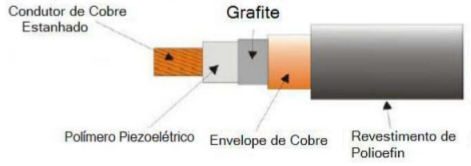
\includegraphics[scale=0.6]{imgs/piezoeletrico.png}
  \end{center}
  \caption{Representação esquemática de um cabo piezoelétrico \citep{goldner:2009:misc}.}
  \label{fig:piezoeletrico}
\end{figure}

Devido a sua grande precisão, esse tipo de sensor é capaz de medir volume do tráfego, velocidade, peso e ainda classificar os veículos baseado no espaçamento e contagem de eixos. Sua instalação é feita junto à via, caracterizando-o como invasivo, e não é recomendado em solos irregulares. Apresenta alto custo se comparado a outros equipamentos invasivos, mas em contrapartida são mais precisos e adquirem informações mais completas.

% section sensores_piezoel_tricos (end)

\subsection{Câmera de vídeo} % (fold)
\label{sub:c_mera_de_v_deo}

As câmeras de vídeo são utilizadas no monitoramento do tráfego, na maioria das vezes, como uma simples ferramenta de vigilância urbana, com capacidades de transmissão e gravação de imagens. Nesse cenário, as imagens devem ser interpretadas por um operador humano, que tem a função de extrair dados de tráfego. Com o avanço das áreas de processamento digital de imagens e visão computacional, surgiram diversos sistemas de gerenciamento do tráfego capazes de extrair automaticamente informações de tráfego importantes, como velocidade, volume, presença, ocupação, densidade, movimentos de conversão, mudança de faixa, aceleração, classificação de veículos e outros \citep{martinsky:2007:masther,feitosa:2012:masther}.

Um sistema inteligente de processamento de imagens de vídeo consiste em uma ou mais câmeras, um \textit{hardware}\footnote{Parte física de computadores ou quaisquer equipamentos eletrônicos.} para digitalização e processamento e um \textit{software} para interpretação e conversão de imagens em dados de tráfego, numéricos ou simbólicos. Segundo \cite{feitosa:2012:masther}, esse tipo de sistema pode, com apenas uma câmera, substituir vários equipamentos invasivos, como laços indutivos, e proporcionar detecção de veículos em múltiplas faixas com menores custos de manutenção.

Dentre as vantagens de uso de câmeras está a instalação, que é totalmente não-invasiva e não gera qualquer tipo de transtorno ao trânsito. Uma vez capturadas, as imagens do tráfego podem ser analisadas posteriormente por profissionais capazes de, por exemplo, realizar a contagem volumétrica manual ou periciar um acidente. Mudanças naturais na cena, como chuvas, tempo nublado, o dia e a noite, podem interferir na visibilidade, dificultando tanto a interpretação humana quanto o processamento digital por visão computacional. Deslocamentos indesejados da câmera e problemas de oclusão também são comuns.

% section c_mera_de_v_deo (end)

\subsection{Sensores micro-ondas} % (fold)
\label{sub:radar_por_microondas}

Esse tipo de equipamento transmite radiação de micro-ondas de baixa energia na direção de uma área do pavimento utilizando uma antena localizada na parte superior do radar. Quando um veículo atravessa um feixe, uma parte dessa energia é refletida de volta para o detector, também localizado na parte superior do radar, e dados como velocidade e presença são calculados por um controlador. A Figura \ref{fig:microondas} ilustra a configuração mais comum de um sistema de monitoramento baseado em sensores micro-ondas.

\begin{figure}[ht]
  \begin{center}
    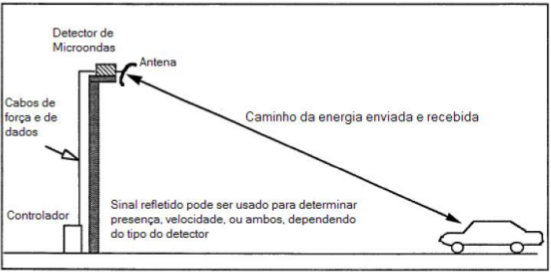
\includegraphics[scale=.6]{imgs/microondas.png}
  \end{center}
  \caption{Esquema ilustrativo da arquitetura de um sistema de monitoramento do tráfego baseado em sensores micro-ondas \citep{goldner:2009:misc}.}
  \label{fig:microondas}
\end{figure}

Esses sensores podem ser de dois tipos:

\begin{itemize}
  \item \textbf{Doppler}: mede a presença de um veículo em função do movimento relativo entre uma fonte sonora e seu receptor e que, por efeito \textit{Doppler}, varia a frequência recebida na volta. Como é um método baseado em movimento, não considera veículos parados ou em regime de ``anda-pára''.
  \item \textbf{Radar}: utiliza um sinal de frequência ou fase modulada para calcular o atraso de tempo da onda refletida, obtendo a distância do veículo. Nesse método é possível detectar a presença de veículos parados, além de medir velocidade, monitorar filas e ocupação.
\end{itemize}

Os sensores micro-ondas são não-invasivos e não interferem no tráfego de veículos no processo de instalação. Geralmente não apresentam sensibilidade em más condições climáticas e podem ser construídos para suportar múltiplas pistas. No entanto, um dos tipos não é capaz de detectar veículos parados.

% section radar_por_microondas (end)

\subsection{Sensores ultrassônicos} % (fold)
\label{sec:sensores_ultrass_nicos}

Esses detectores transmitem ondas de pressão de energia sonora acima da frequência audível humana, que é de 20 KHz. Estas ondas sonoras refletem no pavimento ou no veículo, são captadas por um receptor e processadas para fornecer informações de passagem e presença de veículos. A montagem não-invasiva do equipamento pode ser feita acima ou ao lado da via, como ilustra a Figura \ref{fig:ultrassonico}.

\begin{figure}[ht]
  \begin{center}
    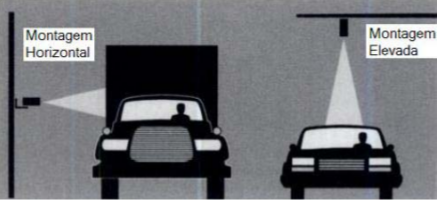
\includegraphics[scale=.65]{imgs/ultrassonico.png}
  \end{center}
  \caption{Tipos de montagem para um sensor ultrassônico \citep{goldner:2009:misc}.}
  \label{fig:ultrassonico}
\end{figure}

Existem dois tipos de sensores ultrassônicos:

\begin{itemize}
  \item \textbf{Pulso ultrassônico}: são emitidos pulsos de energia com largura e período conhecidos. Se o tempo do pulso refletido for menor que o valor conhecido, a presença do veículo é acusada, fornecendo informações de altura, largura, ocupação, volume e classificação.
  \item \textbf{Onda ultrassônica contínua}: usam o princípio  de \textit{Doppler}, que leva em conta a variação da frequência causada pela velocidade relativa entre onda emitida e refletida, para determinar a presença, volume e velocidade veicular.
\end{itemize}

O uso de sensores ultrassônicos é vantajoso pois a instalação é não-invasiva e pode monitorar mais de uma pista ao mesmo tempo. Como desvantagem, as mudanças de temperatura e ventanias podem afetar o seu desempenho.

% section sensores_ultrass_nicos (end)

% section tecnologias_detectoras_de_ve_culos (end)


\section{Aplicações de Visão Computacional} % (fold)
\label{sec:aplica_es_de_vis_o_computacional}

Com o desenvolvimento de pesquisas na área de processamento de imagens digitais nos últimos tempos, impulsionado pelas facilidades de implementação de aplicações de visão computacional utilizando a biblioteca OpenCV \citep{opencv_library}, cada vez mais trabalhos de monitoramento do tráfego que utilizam visão computacional são publicados. A seguir, uma breve revisão bibliográfica de projetos de Engenharia de Transporte que utilizam conceitos de visão computacional.

% \subsection{Direção autônoma de veículo inteligente} % (fold)
% \label{sub:dire_o_aut_noma_de_ve_culo_inteligente}

% \cite{thrun:2006:article}
%TODO: importante por causa do Guilherme

% % subsection dire_o_aut_noma_de_ve_culo_inteligente (end)

% \subsection{Detecção de placa de veículos} % (fold)
% \label{sub:detec_o_de_placa_de_ve_culos}

% \cite{martinsky:2007:masther}

% % subsection detec_o_de_placa_de_ve_culos (end)

\subsection{Contagem volumétrica utilizando dispositivos móveis} % (fold)
\label{sub:contagem_volum_trica_utilizando_dispositivos_m_veis}

\cite{feitosa:2012:masther} propõe em sua Tese de Mestrado em Ciência da Computação pela UFG - Universidade Federal de Goiás, um método para contagem volumétrica de veículos baseado em visão computacional. A pesquisa é focada em otimização de algoritmos de processamento de imagens para execução em dispositivos móveis.

Alguns requisitos são estabelecidos nesse trabalho: as imagens são capturadas da lateral de uma via, com uma câmera fixada em uma baixa altura, identificando e contando veículos que trafegam em ambas as direções; as imagens utilizadas são de baixa resolução; e o processo de contagem é realizado em tempo real.

Apesar de o objetivo do projeto ser a contagem volumétrica via dispositivos móveis, o estudo inicial das técnicas de processamento de imagem e visão computacional é feito em um \textit{laptop}\footnote{Computador portátil, que no Brasil também é conhecido como \textit{notebook}}. A metodologia adotada pode ser dividida em seis etapas principais. São elas:

\begin{enumerate}
  \item \textbf{Entrada de dados}: os \textit{frames}\footnote{Cada um dos quadros de um vídeo.} do vídeo são disponilizados em tempo real ou por um arquivo em disco, que foi gravado anteriormente.
  \item \textbf{Pré-processamento de imagem}: conversão para escala de cinza, caso ainda não esteja nesse formato; equalização do histograma; e suavização da imagem por filtragem linear.
  \item \textbf{Reconhecimento da imagem referência de fundo}: obtenção de um modelo adaptativo da imagem de fundo da cena, utilizando um método de rápido processamento.
  \item \textbf{Definição da área de movimento}: determinação da região da cena com maior movimentação que, provavelmente, é a área de tráfego de veículos. Essa região de interesse também elimina movimentações indesejadas, como por exemplo, o movimento da vegetação.
  \item \textbf{Segmentação de objetos}: subtrai a imagem referência de fundo do \textit{frame} corrente, segmentando os objetos de interesse. Também descarta objetos sem interesse.
  \item \textbf{Acompanhamento de objetos segmentados}: rastreamento dos objetos segmentados ao longo dos quadros, evitando que o mesmo seja contado mais de uma vez.
\end{enumerate}

O método proposto foi implementado em forma de aplicativo na linguagem Java, utilizando a biblioteca de processamento de imagens JavaCV, que utiliza a maior parte das funções da OpenCV \citep{opencv_library}. Como o trabalho de \cite{feitosa:2012:masther} tem por objetivo a execução em dispositivos móveis, o desempenho do algoritmo é um fator determinante. Por isso, foi necessário que alguns algoritmos de processamento de imagens, já existentes na OpenCV, fossem reimplementados com foco em velocidade de execução, o que elevou muito a complexidade do código. Na etapa de reconhecimento da imagem referência de fundo, por exemplo, seria muito mais simples, do ponto de vista de desenvolvimento, utilizar as funções de subtração de \textit{backgroud} já implementadas na OpenCV. No entanto, por ser um método mais completo e complexo, acarretaria em menor desempenho de execução se comparado à implementação de \cite{feitosa:2012:masther}.

Os testes foram realizados a partir de 15 amostras de vídeos, sendo 14 com resolução $640\times 480$ e apenas 1 com resolução $320\times 240$, e duração média de 09:30 minutos. Para avaliar o desempenho do método, num primeiro momento foi feita uma contagem volumétrica manual dos veículos em cada amostra, para que assim o percentual de acerto do método automático, executado no \textit{laptop}, fosse calculado. Além disso, o tempo de execução de cada amostra foi medido.

Em seguida, o aplicativo desenvolvido em Java foi adaptado para ser executado por um dispositivo móvel com sistema operacional Android. Os mesmos testes foram realizados para as 15 amostras e o percentual de acerto permaneceu o mesmo, resultado esperado tendo em vista que os algoritmos de processamento de imagem e visão computacional não mudaram. Nesse novo cenário, o tempo de execução também foi medido. A Tabela \ref{tab:feitosa} lista as medições de cinco amostras.


\begin{table}[ht]
  \caption{Comparação entre resultados de tempo de execução do método pelo \textit{laptop} e celular \citep{feitosa:2012:masther}.}
  \label{tab:feitosa}
  \begin{center}
    \begin{tabular}{ccccc}
    \toprule
    \textbf{Amostra} & \textbf{\% acerto} & \textbf{Duração} & \textbf{Tempo celular} & \textbf{Tempo \textit{laptop}}\\
    \midrule
      1 & 90,58 & 00:15:08 & 01:00:56 & 00:03:54\\
      2 & 92,45 & 00:05:15 & 00:19:55 & 00:01:36\\
      3 & 91,30 & 00:02:44 & 00:11:55 & 00:00:27\\
      4 & 98,15 & 00:10:18 & 00:48:18 & 00:03:39\\
      5 & 97,71 & 00:13:07 & 01:09:27 & 00:03:48\\
    \bottomrule
    \end{tabular}
  \end{center}
\end{table}

Os percentual de acerto obtido nas contagens foi satisfatórios e aplicativo desenvolvido para executar em um \textit{laptop} foi adaptado e portado para um dispositivo móvel Android com sucesso. No entanto, o tempo de execução do método no dispositivo móvel não foi satisfatório, inviabilizando que essa aplicação funcione em tempo real.

% subsection contagem_volum_trica_utilizando_dispositivos_m_veis (end)

% section aplica_es_de_vis_o_computacional (end)
% chapter contagem_de_ve_culos_e_monitoramento_do_tr_fego (end)

\chapter{Visão Computacional} % (fold)
\label{cha:vis_o_computacional}
% !TEX root = pfc.tex

Vis�o computacional, em linhas gerais, � a tecnologia capaz de transformar imagens do mundo real em uma representa��o que computadores s�o capazes de interpretar e processar. Muitos definem vis�o computacional como a ci�ncia das m�quinas que enxergam. � uma base te�rica e tecnol�gica para a constru��o de sistemas artificiais que obt�m informa��es de imagens ou quaisquer dados multidimensionais. Mas como os computadores podem entender o mundo visual dos humanos? Quais vantagens e quais tipos de aplica��es podem existir a partir desse conceito?

O ser humano � perfeitamente capaz de perceber a estrutura tridimensional do mundo ao seu redor. Ao visualizar a Figura \ref{fig:flower}, percebe-se que a vis�o humana interpreta varia��es de transpar�ncia e sombra, al�m de diferenciar o objeto do \textit{backgroud}\footnote{Segundo plano ou plano de fundo} com facilidade \citep{szeliski:2010:book}. Isso acontece porque o c�rebro humano divide o sinal de vis�o em muitos canais, gerando um fluxo de diferentes tipos de informa��o. Ele � capaz de identificar quais s�o as partes importantes de uma imagem a serem examinadas e ao mesmo tempo suprimir a aten��o para regi�es menos importantes. Al�m disso, o c�rebro possui um sistema de realimenta��o poderoso que implementa um controle em malha fechada, composto por sensores (vis�o, audi��o, olfato, tato e paladar) e atuadores (�ris para controlar a entrada de luminosidade nos olhos) \citep{opencv:2008:book}.

\begin{figure}[tb]
  \begin{center}
    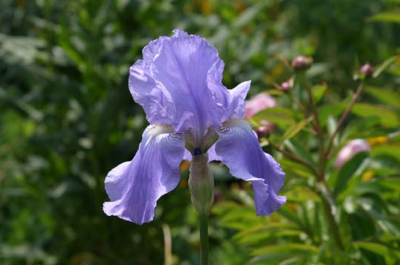
\includegraphics{imgs/flower.png}
  \end{center}
  \caption{O ser humano � capaz de determinar a forma e a transpar�ncia de cada p�tala de uma flor \citep{szeliski:2010:book}.}
  \label{fig:flower}
\end{figure}

Diante dessa facilidade com que o ser humano enxerga o mundo ao seu redor, � intuitivo pensar que o processamento de imagens por vis�o computacional � simples. Mas isso n�o � verdade. Em um sistema de vis�o, o computador recebe, na maioria das vezes, apenas uma matriz de n�meros inteiros, em que cada posi��o � denominada pixel, como mostrado na Figura \ref{fig:opencv_car}. E nada mais! Todos aqueles padr�es de interpreta��o de informa��o presentes no c�rebro n�o existem aqui. Al�m disso, deve-se considerar os ru�dos existentes no sistema que diminuem ainda mais a quantidade de informa��o dos dados. Esse tipo de problema pode ser causado devido a varia��es no ambiente (luminosidade, clima, reflexos, movimenta��es), imperfei��es na captura de imagem (lente, configura��o mec�nica), ru�dos el�tricos no sensor �ptico da c�mera e compress�o das imagens ap�s a captura \citep{opencv:2008:book}.

\begin{figure}[tb]
  \begin{center}
    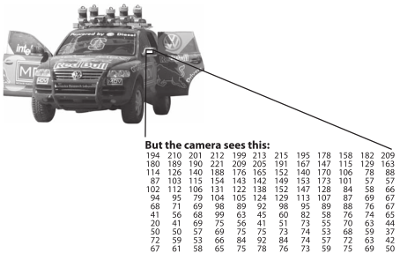
\includegraphics{imgs/opencv_car.png}
  \end{center}
  \caption{Para um computador, o retrovisor de um carro � apenas uma matriz composta por pixeis \citep{opencv:2008:book}.}
  \label{fig:opencv_car}
\end{figure}

Mesmo com todos esses desafios, por incr�vel que pare�a, � poss�vel desenvolver sistemas baseados em vis�o computacional bastante robustos e com alto grau de confiabilidade. Isso come�a a se tornar poss�vel quando as imagens capturadas est�o inseridas no contexto de uma determinada aplica��o. Por exemplo: se um sistema de vis�o computacional tem por objetivo rastrear carros, n�o faz nenhum sentindo buscar os ve�culos em �reas que n�o sejam as ruas, avenidas e rodovias. Caso um objeto seja encontrado em uma �rea verde ou no azul do c�u, a probabilidade de que esse objeto seja um carro � muito baixa. � uma an�lise �bvia mas de suma import�ncia no processamento de imagens.

O uso de m�todos estat�sticos em vis�o computacional tamb�m s�o primordiais, indo de encontro ao problema de ru�dos discutido anteriormente. Considerar a m�dia dos pixeis no tempo � uma abordagem estat�stica, que pode vir a ser uma solu��o para problemas que envolvem imagens ruidosas. Outra t�cnica bastante comum � a constru��o de modelos das c�meras, capazes de caracteriz�-las matematicamente atrav�s de seus par�metros intr�nsecos e extr�nsecos. Os par�metros internos da c�mera como dist�ncia focal, distor��es de lente e tamanho do pixel correspondem aos par�metros intr�nsecos. Os par�metros extr�nsecos est�o relacionados � orienta��o e posi��o da c�mera em rela��o a um sistema de refer�ncia no mundo. Com esses par�metros fica simples corrigir imperfei��es nas imagens, que podem ocorrer devido a lente ou alguma configura��o mec�nica.

Essas e mais uma s�rie de t�cnicas s�o objetos de estudo no campo de vis�o computacional. Elas em conjunto s�o combinadas e organizadas de maneira a transformar quaisquer dados multidimensionais em informa��es de alto n�vel, como por exemplo aus�ncia e presen�a de um componente, dimens�o e cor de objetos. Como regra geral: quanto mais restrito � o escopo de uma aplica��o de vis�o computacional, mais o problema pode ser simplificado e mais confi�vel ser� a solu��o final \citep{opencv:2008:book}.

A seguir � realizado uma breve revis�o bibliogr�fica sobre conceitos, t�cnicas e m�todos de processamento de imagens digitais aplicados ao campo da vis�o computacional.

\section{Imagem digital} % (fold)
\label{sec:imagem_digital}

% section imagem_digital (end)

\section{Espa�os de cor} % (fold)
\label{sec:espa_os_de_cor}

% section espa_os_de_cor (end)

\section{Escala de cinza} % (fold)
\label{sec:escala_de_cinza}

% section escala_de_cinza (end)

\section{Filtros} % (fold)
\label{sec:filtros}

% section filtros (end)

\section{Limiariza��o} % (fold)
\label{sec:limiariza_o}

% section limiariza_o (end)

\section{Subtra��o de fundo} % (fold)
\label{sec:subtra_o_de_background}

% section subtra_o_de_background (end)

\section{Opera��es morfol�gicas} % (fold)
\label{sec:opera_es_morfol_gicas}

\subsection{Eros�o} % (fold)
\label{sub:eros_o}

\subsection{Dilata��o} % (fold)
\label{sub:dilata_o}

\subsection{Abertura e fechamento} % (fold)
\label{sub:abertura_e_fechamento}

% subsection abertura_e_fechamento (end)

% subsection dilata_o (end)

% subsection eros_o (end)

% section opera_es_morfol_gicas (end)

\section{Detec��o de caracter�sticas relevantes} % (fold)
\label{sec:detec_o_de_caracter_sticas_relevantes}

% section detec_o_de_caracter_sticas_relevantes (end)

\section{Biblioteca OpenCV} % (fold)
\label{sec:biblioteca_opencv}

OpenCV (\textit{Open Source Computer Vision}) \citep{opencv_library} � uma biblioteca de vis�o computacional \textit{open source}\footnote{Veja em: \url{http://opensource.org}} dispon�vel em: \url{http://sourceforge.net/projects/opencvlibrary/}. O c�digo � escrito em C e C++ e pode ser compilado e executado em ambientes Linux, Windows e Mac OS X. Existem tamb�m interfaces em Python, Ruby, Matlab e outras linguagens. Cont�m mais de 500 algoritmos otimizados para processamento de imagens e v�deos, cobrindo diversas �reas da vis�o computacional, como: inspe��o industrial, imagens m�dicas, seguran�a, interface com o usu�rio, calibra��o de c�mera, vis�o est�reo, rob�tica e \textit{machine learning} \citep{opencv:2008:book}.

Segundo \citeauthor{opencv2:2011:book}, desde seu lan�amento em 1999 ela vem sendo largamente adotada como a principal ferramenta de desenvolvimento pela comunidade de pesquisadores e programadores em vis�o computacional. OpenCV foi originalmente desenvolvida pela Intel \citep{intel:2013:online}, por um time liderado por Gary Bradski e com o prop�sito de avan�ar em pesquisas na �rea de vis�o. Depois de uma s�rie de vers�es \textit{Beta}, a vers�o 1.0 foi lan�ada em 2006. O segundo maior lan�amento aconteceu em 2009 com a OpenCV 2, propondo importantes modifica��es em sua estrutura e especialmente a nova interface C++. Atualmente a OpenCV encontra-se na vers�o 2.4.

\citeauthor{opencv:2008:book} afirmam que a licen�a \textit{open source} da OpenCV permite que aplica��es comerciais possam ser construidas utilizando parte ou toda a biblioteca, sem a necessidade de que o c�digo da aplica��o seja aberto. Devido a essa pol�tica liberal de uso, gigantes como IBM, Microsoft, Intel, SONY, Siemens, Google e outros, al�m dos centros de pesquisa Stanford, MIT, CMU, Cambridge, INRIA e outros, utilizam a biblioteca em seus projetos e pesquisas. A OpenCV foi pe�a chave no sistema de vis�o de um rob� desenvolvido em Stanford, conhecido como Stanley, que ganhou a corrida de carros aut�nomos \$2M DARPA Grand Challenge \citep{thrun:2006:article}.

% section biblioteca_opencv (end)

\section{Aplica��es existentes} % (fold)
\label{sec:aplica_es_existentes}

Diversos tipos de aplica��o podem ser concebidas utilizando os conhecimentos de vis�o computacional. O fato dessa tecnologia ser n�o intrusiva, ou seja, n�o altera em nada o meio em que est� sendo utilizada, torna os sistemas de vis�o realiz�veis em grande parte dos processos industriais, urbanos e ambientais \citep{ivision:2013:online}.

\subsection{An�lise dimensional} % (fold)
\label{sub:an_lise_dimensional}

As aplica��es em an�lise dimensional se caracterizam por efetuarem medidas em objetos, sendo elas lineares e/ou angulares. A an�lise dimensional por imagem � vantajosa pois possibilita que as medidas sejam feitas � dist�ncia, quando n�o � poss�vel ou desej�vel o contato direto com o objeto. C�meras de alta resolu��o se aplicam nesses projetos, garantindo medi��es precisas e com repetibilidade. Muito comum na siderurgia, esse tipo de aplica��o possibilita a medi��o em objetos que se encontram em altas temperaturas. As c�meras infravermelho tem sido utilizadas nesse tipo de aplica��o.

% subsection an_lise_dimensional (end)

\subsection{Reconhecimento de padr�es} % (fold)
\label{sub:reconhecimento_de_padr_es}

O uso de reconhecimento de padr�es permite a identifica��o de caracter�sticas de um produto comparando-o com um modelo predeterminado. Essas caracter�sticas a serem inspecionadas s�o escolhidas de modo a identificar e diferenciar um tipo de modelo de outro. Assim � poss�vel dizer se um objeto est� conforme um padr�o ou n�o.

% subsection reconhecimento_de_padr_es (end)

\subsection{Inspe��o de n�vel} % (fold)
\label{sub:inspe_o_de_n_vel}

Esse tipo de aplica��o � bastante comum na ind�stria de bebidas e na ind�stria farmac�utica para inspe��o de enchimento de ampolas, vidros de medicamentos ou qualquer recipiente transl�cido que contenha l�quido.

% subsection inspe_o_de_n_vel (end)

\subsection{Inspe��o por an�lise de cores} % (fold)
\label{sub:inspe_o_por_an_lise_de_cores}

Possibilita a cria��o de solu��es para separar produtos por cor ou verificar se a tonalidade est� igual a uma amostra. Tem a vantagem de ser um m�todo determin�stico em rela��o a uma inspe��o de cores realizada por seres humanos, onde pode existir subjetividade. No entanto, varia��es de luminosidade podem dificultar a realiza��o desse tipo de inspe��o.

% subsection inspe_o_por_an_lise_de_cores (end)

\subsection{Rastreabilidade} % (fold)
\label{sub:rastreabilidade}

S�o aplica��es de leituras de c�digos de barras ou de c�digos bidimensionais como \textit{Data Matrix}\footnote{C�digo de barras matricial bi-dimensional que consiste em c�lulas brancas ou pretas arranjadas em forma de quadrado ou ret�ngulo. Se caracteriza pelas bordas em formato de L. Armazena no m�ximo 2335 caracteres alfanum�ricos.} e o \textit{QR Code}\footnote{\textit{Quick Response Code} � um c�digo de barras bi-dimensional criado pela empresa japonesa Denso-Wave em 1994. Pode armazenar at� 7089 caracteres, dependendo do tipo de dado. Possui redund�ncia em sua codifica��o, possibilitando corre��o e recupera��o de informa��o.}. Permitem identificar e rastrear os produtos, bem como armazenar grandes quantidades de dado. S�o sistemas frequentemente utilizados na ind�stria automobil�stica mas s�o aplic�veis em qualquer projeto que necessite de controle de produ��o.

% subsection rastreabilidade (end)

\subsection{Contagem, Sele��o e Classifica��o} % (fold)
\label{sub:contagem_sele_o_e_classifica_o}

As aplica��es para contagem, sele��o e classifica��o podem instrumentar diversas ind�strias, como por exemplo a ind�stria farmac�utica para contagem de medicamentos. Tamb�m � comum na produ��o de componentes eletr�nicos para verifica��o de pinos e conectores. Na engenharia de transporte podem contribuir na an�lise do tr�fego realizando contagem volum�trica de ve�culos e pessoas.

% subsection contagem_sele_o_e_classifica_o (end)

% section aplica_es_existentes (end)


% chapter vis_o_computacional (end)

\chapter{Metodologia} % (fold)
\label{cha:metodologia}
% !TEX root = pfc.tex


Como visto no Cap�tulo \ref{cha:vis_o_computacional}, existem diversas t�cnicas de processamento digital de imagens que possibilitam que aplica��es de vis�o computacional sejam capazes de extrair informa��es a partir de uma ou mais imagens de entrada.

\begin{figure}[ht]
  \begin{center}
    \begin{subfigure}[b]{.49\textwidth}
      \begin{center}
        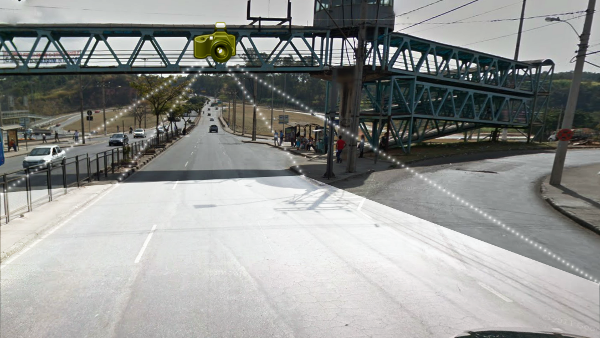
\includegraphics[width=1\linewidth]{imgs/cena_captura.png}
      \end{center}
      \caption{}
      \label{fig:cena_captura}
    \end{subfigure}
    \begin{subfigure}[b]{.49\textwidth}
      \begin{center}
        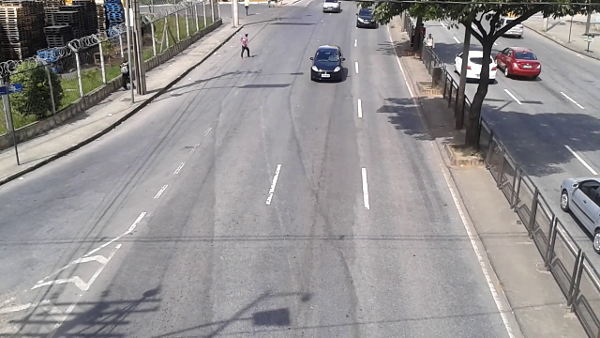
\includegraphics[width=1\linewidth]{imgs/original_frame.png}
      \end{center}
      \caption{}
      \label{fig:original_frame}
    \end{subfigure}
  \end{center}
  \caption{(a) Posicinamento da c�mera para captura de imagens. A �rea em destaque simboliza }
  \label{fig:cena}
\end{figure}


\begin{figure}[ht]
  \begin{center}
    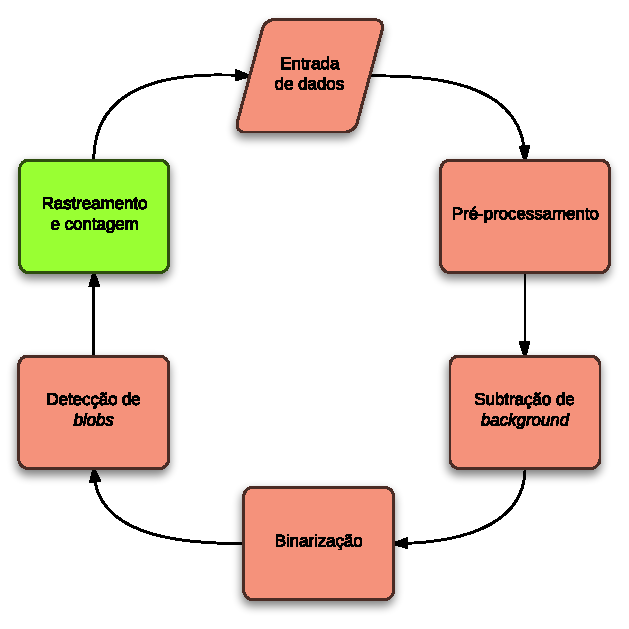
\includegraphics[scale=0.9]{imgs/general_process.pdf}
  \end{center}
  \caption{Fluxograma com a representa��o global do m�todo de contagem.}
  \label{fig:general_process}
\end{figure}

\section{Entrada de dados} % (fold)
\label{sec:entrada_de_dados}

\begin{lstlisting}
#include <iostream>

#include <opencv2/core/core.hpp>
#include <opencv2/highgui/highgui.hpp>
#include <opencv2/imgproc/imgproc.hpp>

int main(int argc, char const *argv[])
{
  cv::VideoCapture capture;
  if(!capture.isOpened()) {
    std::cout << "can not open camera or video file" << std::endl;
    return;
  }
  ...  
  for(;;) {
    cv::Mat frame;
    capture >> frame;

    if(frame.empty()) break; 
    ...  
  }

  return 0;
}
\end{lstlisting}

% section entrada_de_dados (end)

\section{Pr�-processamento} % (fold)
\label{sec:pr_processamento}

\begin{lstlisting}
  ...
  for(;;) {
    ...
    cv::Mat gray;
    cv::cvtColor(frame, gray, CV_BGR2GRAY);

    cv::GaussianBlur(gray, gray, cv::Size(7, 7), 3);
    ...
  }
  ...  

\end{lstlisting}

% section pr_processamento (end)

\section{Subtra��o de \textit{background}} % (fold)
\label{sec:subtra_o_de_background}

\begin{lstlisting}
  ...
  cv::BackgroundSubtractorMOG2 model;
  for(;;) {
    ...
    cv::Mat foreground;
    model(gray, foreground);
    ...
  }
  ...
\end{lstlisting}

% section subtra_o_de_i (end)

\section{Binariza��o} % (fold)
\label{sec:binariza_o}

\begin{lstlisting}

void bin(cv::Mat &src)
{
    //conta os pixeis cinza
    int sumGray = 0, sumWhite = 0;
    for(int i = 0; i < src.rows; i++) {
        const uchar* ptri = src.ptr<uchar>(i);
        for(int j = 0; j < src.cols; j++) {
            if(ptri[j] != 0 && ptri[j] != 255)
                sumGray++;
            else if(ptri[j] == 255)
                sumWhite++;
        }
    }

    if(sumWhite == 0) {
        src.setTo(cv::Scalar(0));
    }
    else if((float)sumGray/(float)sumWhite > 10.0)
        cv::threshold(src, src, 250, 255, CV_THRESH_BINARY);
    else
        cv::threshold(src, src, 5, 255, CV_THRESH_BINARY);
}

  ...
  for(;;) {
    ...
    bin(foreground);

    cv::Mat morph;
    cv::Mat element = cv::getStructuringElement(cv::MORPH_ELLIPSE,
                                                cv::Size(5,5));
    cv::morphologyEx(foreground, morph, CV_MOP_CLOSE, element, 
                     cv::Point(-1,-1), 3);
    ...
  }
  ...  
\end{lstlisting}

% section binariza_o (end)

\section{Detec��o de \textit{blobs}} % (fold)
\label{sec:detec_o_de_blobs}

\begin{lstlisting}
  ...
    cv::SimpleBlobDetector::Params params;
    params.filterByInertia = false;
    params.filterByConvexity = false;
    params.filterByColor = true;
    params.blobColor = 255;
    params.filterByCircularity = false;
    params.filterByArea = true;
    params.minArea = 500.0f;
    params.maxArea = 80000.0f;

    cv::Ptr<cv::FeatureDetector> detector = 
                                 new cv::SimpleBlobDetector(params);
    ...
    for(;;) {
      ...
      std::vector<cv::KeyPoint> keypoints;
      detector.detect(morph, keypoints)
    }
    ... 
  
\end{lstlisting}

% section detec_o_de_textit_ (end)

\section{Rastreamento e contagem} % (fold)
\label{sec:rastreamento_e_contagem}

\begin{figure}[ht]
  \begin{center}
    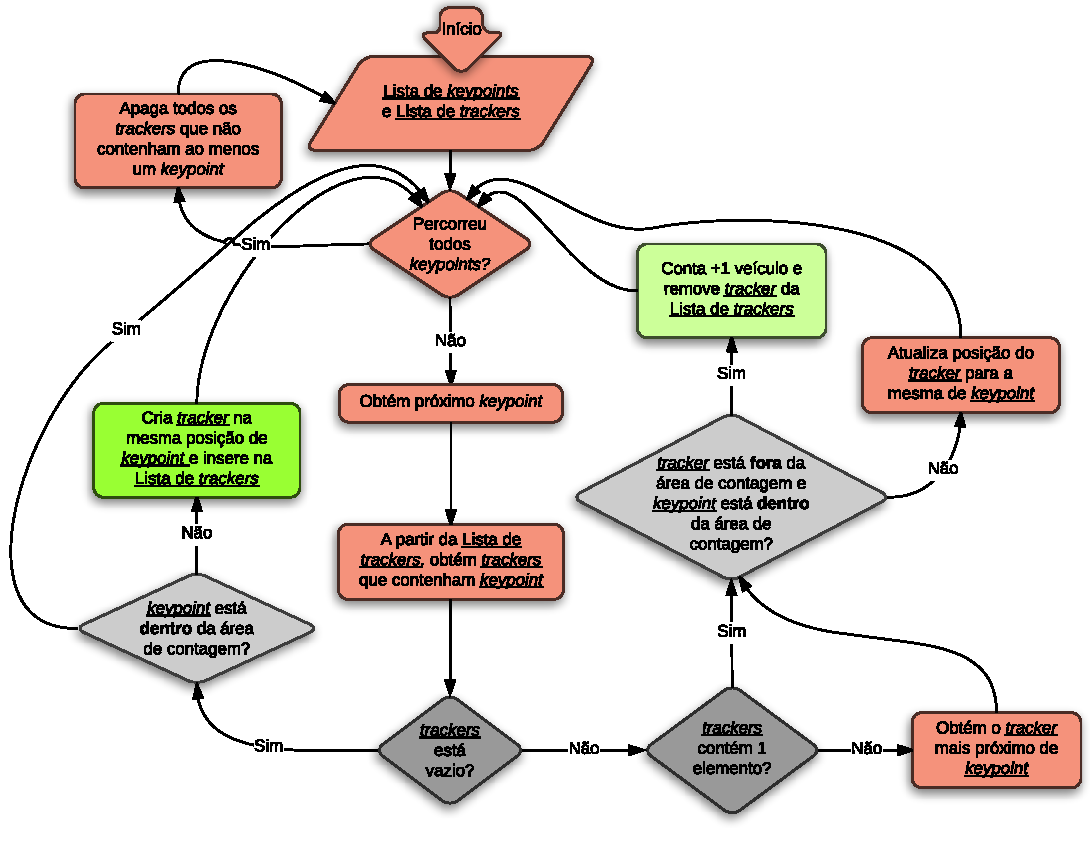
\includegraphics[scale=0.85]{imgs/fluxograma_contagem.pdf}
  \end{center}
  \caption{Fluxograma do m�todo de rastreamento de \textit{keypoints} utilizando \textit{trackers} e contagem de ve�culos.}
  \label{fig:fluxograma_contagem}
\end{figure}

% section rastreamento_e_contagem (end)
% chapter metodologia (end)

\chapter{Testes e Resultados} % (fold)
\label{cha:testes_e_resultados}
% !TEX root = pfc.tex

O método proposto foi implementado em forma de um \textit{software} multiplataforma, desenvolvido em linguagem \verb!C++! \citep{cplusplus:2013:online}, com intuito de obter um bom desempenho de execução e fácil implementação utilizando os conceitos de programação orientada a objetos.

Como biblioteca para processamento das imagens, foi utilizado a OpenCV 2.4.4 \citep{opencv_library}, contribuindo para que operações complexas de visão computacional pudessem ser realizadas com poucas linhas de código. O desenvolvimento do método não está preso à tecnologia escolhida, podendo ser empregado utilizando outras linguagens de programação, bem como outras bibliotecas. A tecnologia foi escolhida visando a simplicidade no processo de desenvolvimento das operações de processamento de imagens, que estão bem detalhadas pelos trechos de código na Seção \ref{sec:fluxo_de_processos}.

\section{Testes} % (fold)
\label{sec:testes}

Todos os vídeos foram capturados por um aparelho celular Samsung OMNIA W GT-I8350 \citep{omnia:2013:online}, como descrito na Seção \ref{sec:caracter_sticas_de_captura}. As imagens foram feitas na passarela localizada na Av. Presidente Carlos Luz, nos dois sentidos da via, como ilustra a Figura \ref{fig:sentidos}. Duas configurações de captura foram utilizadas:

\begin{itemize}
  \item HD 720p: gerando vídeos com resolução $1280\times 720$, e \textit{framerate} de 29 FPS;
  \item VGA: gerando vídeos com resolução $640\times 480$, e \textit{framerate} de 29 FPS.
\end{itemize}

Com intuito de equiparar as resoluções dos vídeos gerados a partir das duas configurações de captura, as amostras em HD foram redimensionadas para ter altura e largura metade do valor original, resultando em vídeos com resolução $640\times 360$. A Tabela \ref{tab:videos_teste} lista as amostras utilizadas.

% \noindent Uma terceira resolução foi obtida a partir dos vídeos em HD, aplicando uma operação para redimensioná-los com altura e largura a metade do valor original. Essas variações de cena e resolução foram feitas com o objetivo de avaliar o comportamento do método em diferentes condições. Assim, será possível identificar o impacto de cada variável no resultado final. A Tabela \ref{tab:videos_teste} lista as amostras utilizadas.

\begin{figure}[ht]
  \begin{center}
    \begin{subfigure}[b]{.49\textwidth}
      \begin{center}
        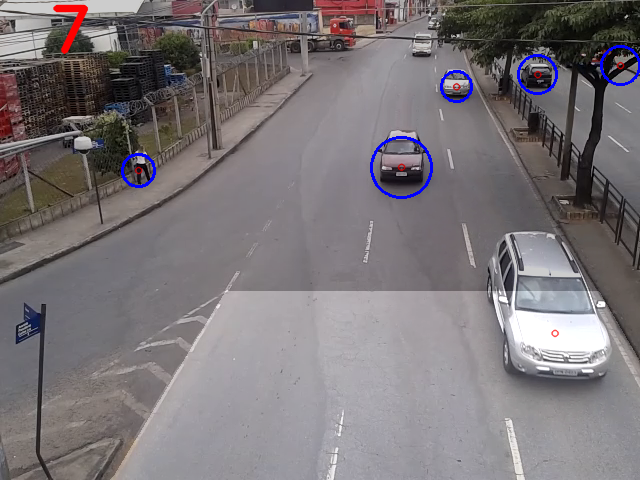
\includegraphics[width=1\linewidth]{imgs/trackers.png}
      \end{center}
      \caption{}
      \label{fig:sentido_pampulha}
    \end{subfigure}
    \begin{subfigure}[b]{.49\textwidth}
      \begin{center}
        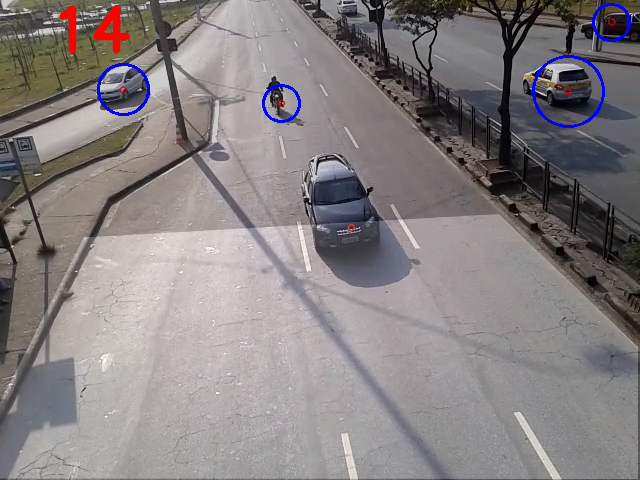
\includegraphics[width=1\linewidth]{imgs/sentido_centro.png}
      \end{center}
      \caption{}
      \label{fig:sentido_centro}
    \end{subfigure}
  \end{center}
  \caption{Resultado do método de contagem para dois tipos de cena. (a) Av. Carlos Luz, sentido Pampulha; (b) Av. Carlos Luz, sentido Centro.}
  \label{fig:sentidos}
\end{figure}

\begin{table}[ht]
  \caption{Vídeos utilizados nos testes.}
  \label{tab:videos_teste}
  \begin{center}
    \begin{tabular}{clcccc}
    \toprule
    \textbf{Nº} & \textbf{Nome do vídeo} & \textbf{Resolução} & \textbf{Duração} & \textbf{FPS} \\
    \midrule
      1 & carlos\_luz\_centro\_vga & $ 640\times 480 $ & 00:05:23 & 29 \\
      2 & carlos\_luz\_centro\_hd\_resized & $ 640\times 360 $ & 00:05:25 & 29 \\
      % carlos\_luz\_centro\_hd & $ 1280\times 720 $ & 00:05:29 & 29 \\
      3 & carlos\_luz\_pampulha\_vga\_1 & $ 640\times 480 $ & 00:05:43 & 29 \\
      4 & carlos\_luz\_pampulha\_vga\_2 & $ 640\times 480 $ & 00:05:19 & 29 \\
      5 & carlos\_luz\_pampulha\_hd\_2\_resized & $ 640\times 360 $ & 00:06:19 & 29 \\
      % carlos\_luz\_pampulha\_hd\_2 & $ 1280\times 720 $ & 00:06:21 & 29 \\
    \bottomrule
    \end{tabular}
  \end{center}
\end{table}

Tanto o desenvolvimento do \textit{software}, quanto os testes, foram feitos em um \textit{Laptop} Dell Vostro V131, Processador Intel Core I3-2330M (2.20GHZ, dual core 4 Threads, 3MB L3 cache), 8GB de memória RAM, em ambiente Linux Fedora 18 (Spherical Cow).

% section testes (end)

\section{Resultados e discussão} % (fold)
\label{sec:resultados_e_discuss_o}

\begin{table}[ht]
  \caption{Matriz de confusão e Índice Kappa (K).}
  \label{tab:matrix_result}
  \begin{center}
    \begin{tabular}{c|cccc|cccccc|cc}
    \toprule
    \textbf{Nº} & \textbf{VP} & \textbf{VN} & \textbf{FP} & \textbf{FN} & \textbf{E} & \textbf{VPN} & \textbf{P} & \textbf{R} & \textbf{FM} & \textbf{A} & \textbf{K} & \textbf{Qual.} \\
    \midrule
      1 & 92 & 35 & 2 & 6 & 0.95 & 0.85 & 0.98 & 0.94 & 0.96 & 0.94 & 0.86 & Excelente\\
      2 & 76 & 34 & 6 & 10 & 0.85 & 0.77 & 0.93 & 0.88 & 0.90 & 0.87 & 0.71 & Muito bom\\
      3 & 107 & 19 & 1 & 26 & 0.95 & 0.42 & 0.99 & 0.80 & 0.89 & 0.82 & 0.49 & Bom \\
      4 & 87 & 28 & 8 & 22 & 0.78 & 0.56 & 0.92 & 0.80 & 0.85 & 0.79 & 0.51 & Bom \\
      5 & 94 & 37 & 2 & 15 & 0.95 & 0.71 & 0.98 & 0.86 & 0.92 & 0.89 & 0.73 & Muito bom\\
    \bottomrule
    \end{tabular}
  \end{center}
\end{table}

\begin{figure}[ht]
  \begin{center}
    \begin{subfigure}[b]{.49\textwidth}
      \begin{center}
        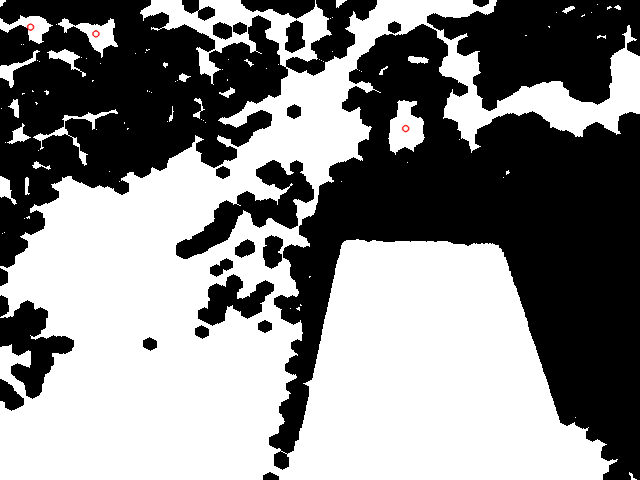
\includegraphics[width=1\linewidth]{imgs/problema_veiculo_grande.png}
      \end{center}
      \caption{}
      \label{fig:problema_veiculo_grande}
    \end{subfigure}
    \begin{subfigure}[b]{.49\textwidth}
      \begin{center}
        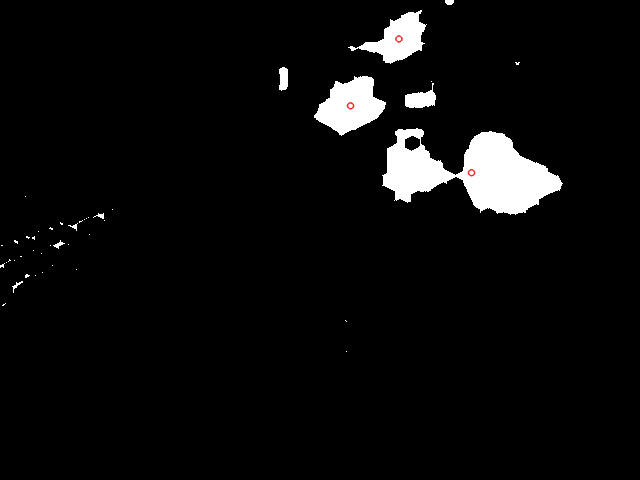
\includegraphics[width=1\linewidth]{imgs/problema_veiculo_junto.png}
      \end{center}
      \caption{}
      \label{fig:problema_veiculo_junto}
    \end{subfigure}
  \end{center}
  \caption{Problemas encontrados no processamento de imagens. (a) A operação de subtração de \textit{background} fica comprometida quando veículos com área muito grande aparecem na cena. (b) Veículos próximos são detectados como um único objeto, definindo apenas um \textit{keypoint}.}
  \label{fig:problemas}
\end{figure}

% section resultados_e_discuss_o (end)

% \section{Resultados finais} % (fold)
% \label{sec:resultados_finais}


% Na Tabela \ref{tab:resultados_contagem} são apresentados os resultados obtidos pela contagem via métodos manual e automático, indicando o percentual de acerto para cada amostra. É importante destacar que o resultado da contagem automática representa o total de veículos identificados na amostra, incluindo falsos positivos e descartando objetos detectados ou rastreados incorretamente. Portanto, os percentuais de acerto são medições estatísticas, que representam apenas o desvio existente entre o valor real e o valor medido.

% \begin{table}[ht]
%   \caption{Resultados de contagem volumétrica.}
%   \label{tab:resultados_contagem}
%   \begin{center}
%     \begin{tabular}{l|cccc}
%     \toprule
%     \textbf{Nome do vídeo} & \textbf{Resolução} & \textbf{Manual} & \textbf{Autom.} & \textbf{\% acerto}\\
%     \midrule
%       carlos\_luz\_centro\_vga & $ 640\times 480 $ & 164 & 156 & 95,12 \\
%       carlos\_luz\_centro\_hd\_resized & $ 640\times 360 $ & 150 & 153 & 98,04 \\
%       carlos\_luz\_centro\_hd & $ 1280\times 720 $ & 150 & 145 & 96,67 \\
%       carlos\_luz\_pampulha\_vga\_1 & $ 640\times 480 $ & 208 & 173 & 83,17 \\
%       carlos\_luz\_pampulha\_vga\_2 & $ 640\times 480 $ & 169 & 138 & 81,66 \\
%       carlos\_luz\_pampulha\_hd\_2\_resized & $ 640\times 360 $ & 201 & 175 & 87,06 \\
%       carlos\_luz\_pampulha\_hd\_2 & $ 1280\times 720 $ & 201 & 170 & 84,58 \\
%     \bottomrule
%     \end{tabular}
%   \end{center}
% \end{table}

% Percebe-se que para uma mesma cena, a variação da resolução do vídeo não afeta de forma siginificativa o percentual de acerto, mostrando que vídeos de alta resolução não trazem vantagens nesse tipo de aplicação. Já a mudança da cena alterou o resultado. Nas amostras do tráfego no sentido centro o percentual de acerto foi superior a 95\%, enquanto que as imagens do outro sentido não ultrapassaram os 90\%. 

% Analisando os vídeos é possível identificar vários veículos de grande porte trafegando no sentido Pampulha, muitos saindo da Fábrica da Coca-Cola ali localizada. Esses objetos com área muito grande causam problemas na etapa de subtração de \textit{background}, como mostrado na Figura \ref{fig:problema_veiculo_grande}, interferindo por alguns \textit{frames} no processo de detecção de \textit{blobs} e gerando oclusão em veículos menores. 

% Esse tipo de tráfego na cena fez com que o resultado da contagem automática ficasse sempre abaixo da referência em todas as amostras sentido Pampulha, justificando o percentual de acerto baixo.


% Outro tipo de problema acontece na etapa de detecção de \textit{blobs}, ilustrado na Figura \ref{fig:problema_veiculo_junto}. Nessa situação, dois veículos próximos foram identificados como um único objeto e apenas um \textit{keypoint} foi definido. Portanto, apenas um \textit{tracker} foi criado e um único veículo contado nesse caso.

% Para avaliar o desempenho computacional do método adotado, mediu-se o tempo de execução do algoritmo para cada uma das amostras, como mostra a Tabela \ref{tab:resultados_tempo}. Percebe-se que a resolução do vídeo está diretamente relacionada ao tempo gasto no processamento. Os vídeos em HD foram processados com mais de três vezes o tempo de processamento dos vídeos em VGA, inviabilizando a utilização dessa configuração em aplicações de tempo real. Os vídeos redimensionados, com resolução $ 640\times 360 $, gastaram menos tempo de processamento do que sua própria duração, indicando que a contagem em tempo real nesse caso seria viável.

% Com intuito de manter o algoritmo simples e o mais genérico possível, os \textit{frames} são processados por completo, sem considerar regiões de interesse. A definição de regiões de interesse, também conhecidas como ROI's\footnote{\textit{Region of interest}}, é um recurso muito utilizado em visão computacional. Quando usado, apenas as porções da imagem que contenham informações relevantes são consideradas no processamento, reduzindo o tempo e o custo computacional.

% \begin{table}[ht]
%   \caption{Tempo real gasto na execução do método de contagem.}
%   \label{tab:resultados_tempo}
%   \begin{center}
%     \begin{tabular}{lccc}
%     \toprule
%     \textbf{Nome do vídeo} & \textbf{Resolução} & \textbf{Duração} & \textbf{Tempo gasto} \\
%     \midrule
%       carlos\_luz\_centro\_vga & $ 640\times 480 $ & 00:05:23 & 00:05:47 \\
%       carlos\_luz\_centro\_hd\_resized & $ 640\times 360 $ & 00:05:25 & 00:05:16 \\
%       carlos\_luz\_centro\_hd & $ 1280\times 720 $ & 00:05:29 & 00:17:48 \\
%       carlos\_luz\_pampulha\_vga\_1 & $ 640\times 480 $ & 00:05:43 & 00:06:04 \\
%       carlos\_luz\_pampulha\_vga\_2 & $ 640\times 480 $ & 00:05:19 & 00:05:33 \\
%       carlos\_luz\_pampulha\_hd\_2\_resized & $ 640\times 360 $ & 00:06:19 & 00:05:38 \\
%       carlos\_luz\_pampulha\_hd\_2 & $ 1280\times 720 $ & 00:06:21 & 00:19:00 \\
%     \bottomrule
%     \end{tabular}
%   \end{center}
% \end{table}

% section resultados_finais (end)
% chapter testes_e_resultados (end)

\chapter{Considerações Finais} % (fold)
\label{cha:considera_es_finais}
% !TEX root = pfc.tex

Baseado nos estudos das t�cnicas de processamento de imagens e trabalhos de vis�o computacional com objetivos semelhantes, foi criado um m�todo de simples implementa��o que realiza a segmenta��o e o acompanhamento de objetos, tornando assim poss�vel a contagem volum�trica dos mesmos. Em todas as amostras, mostradas na Tabela \ref{tab:resultados_contagem}, a contagem realizada se mostrou satisfat�ria.

O desempenho do algoritmo para as amostras em HD foi baixo, inviabilizando a execu��o em tempo real. No ambiente de testes utilizado, descrito na Se��o \ref{sec:testes}, apenas os v�deos com resolu��o $640\times 360$ poderiam ser utilizados para processamento em tempo real. Com um poder de processamento maior, provavelmente seria poss�vel realizar a contagem em tempo real nos v�deos com resolu��o $640\times 480$.

Embora j� existam diversos m�todos para a realiza��o de contagem volum�trica de ve�culos, como descrito no Cap�tulo \ref{cha:contagem_de_ve_culos_e_monitoramento_do_tr_fego}, geralmente eles s�o muito caros e causam transtornos na via durante sua instala��o e manuten��o. O trabalho em quest�o prop�e um m�todo n�o-invasivo, de baixo custo e simples implementa��o, capaz de obter medi��es de boa precis�o.

\section{Limita��es} % (fold)
\label{sec:pontos_negativos_do_m_todo}

V�rios aspectos de altera��o din�mica da cena interferiram no processamento digital. O algoritmo de subtra��o de \textit{background}, por exemplo, apresentou problemas quando ve�culos de grande porte aparecem nas imagens, como mostra a Figura \ref{fig:problema_veiculo_grande}. 

Como n�o foi desenvolvido um m�todo para identificar se o objeto em movimento � um veiculo ou n�o, alguns elementos indesej�veis foram considerados na contagem. Ao mesmo tempo, devido � proximidade, a detec��o de \textit{blobs} falhou e alguns ve�culos n�o foram contabilizados, como mostrado na Figura \ref{fig:problema_veiculo_junto}.

% section pontos_negativos_do_m_todo (end)

\section{Trabalhos futuros} % (fold)

Como poss�veis trabalhos futuros, podem ser apontados:

\begin{itemize}
  \item Defini��o de uma uma regi�o de interesse baseada na �rea com maior movimenta��o nas imagens;
  \item Desenvolvimento de um m�todo para contagem de ve�culos no per�odo noturno ou em locais com baixa ilumina��o;
  \item Cria��o de t�cnicas para classifica��o de ve�culos quanto ao tamanho;
  \item Contagem de ve�culos em cruzamentos, com deslocamentos em v�rias dire��es e sentidos;
  \item Estima��o do volume do tr�fego em vias congestionadas.
\end{itemize}

\label{sec:trabalhos_futuros}

% section trabalhos_futuros (end)
% chapter considera_es_finais (end)

% Aqui vem a parte da bibliografia: use o comando \ppgccbibliography indicando
% apenas o nome do arquivo .bib (sem a extensão).
\ppgccbibliography{bibfile}


% Este comando encapsula o conjunto de apêndices. A sua função é fazer com que
% a numeração dos apêndices seja feita com letras maiúsculas (A, B, C, etc.) e
% a palavra "Apêndice" anteceda as entradas no Sumário.
% \begin{appendices}

% Para cada apêndice, um \chapter
% \chapter{Um apêndice}
% \chapter{Outro apêndice}

% Fim dos apêndices (usar apenas depois do último apêndice)
% \end{appendices}


% Este comando encapsula o conjunto de anexos. A sua função é fazer com que a
% numeração dos anexos seja feita com letras maiúsculas (A, B, C, etc.) e a
% palavra "Anexo" anteceda as entradas no Sumário.
% \begin{attachments}

% Para cada anexo, um \chapter
% \chapter{Um anexo}
% \chapter{Outro anexo}

% Fim dos anexos (usar apenas depois do último anexo)
% \end{attachments}


\end{document}
